\section{SELU ByteNet}

The simplified ByteNet experiments indicate that the compression and decompression layers are necessary and the normalization layers are very expensive. From these observations, it makes sense to analyze whether or not the normalization layers are necessary for the network to converge.

The experiment in figure \ref{fig:result:selu-bytenet:bytenet-nonorm-wmt} is the ``Memorizing WMT NewsTest'' experiment on the ByteNet model without normalization layers. The experiment ran for 300 epochs.

\begin{figure}[h]
    \centering
    \includegraphics[scale=1]{bytenet-nonorm/validation-memorize-wmt.pdf}
    \caption{Shows BLEU score and cross entropy loss for the German to English WMT NewsTest dataset using the ByteNet model without any normalization layers. The exponential moving average used a forget factor of $0.1$.}
    \label{fig:result:selu-bytenet:bytenet-nonorm-wmt}
\end{figure}

Figure \ref{fig:result:selu-bytenet:bytenet-nonorm-wmt} shows that the non-normalized ByteNet model never completely memorizes the training dataset as it should. This is likely due to a vanishing gradient issue, that causes it to converge very slowly. It is possible that it could still learn actual translation when trained on the Europarl v7 dataset, however, it is not very likely.

Recently a new paper showed that it is possible to create a ``self-normalizing neural network''. This means that normalization isn't done explicitly by a normalization layer, but instead, the network is created such that the parameters will converge to weights that ensure normalized internal values.

The ``self-normalizing neural network'' was achieved by using a different activation function and weight initialization. Primarily it is the activation function that is responsible for making the network \textit{self-normalizing}. The initialization is just to ensure a reasonable starting point, as the ``self-normalizing neural network'' is only able to ``self-normalize'' given a reasonable starting variance and mean. \cite{selu}.

The activation function is a variation on the exponential-linear-unit (ELU), which is similar to the ReLU activation function. The difference from ELU is that two constants ($\lambda, \alpha$) are added:
\begin{equation}
\mathrm{SELU}(x) = \lambda \begin{cases}
  x & x > 0 \\
  \alpha (\mathrm{exp}(x) - 1) & x \le 0
\end{cases},\quad \text{where: } \begin{array}{c}
  \alpha = 1.6732632423 \\
  \lambda = 1.0507009873
\end{array}
\end{equation}

\begin{figure}[h]
    \centering
    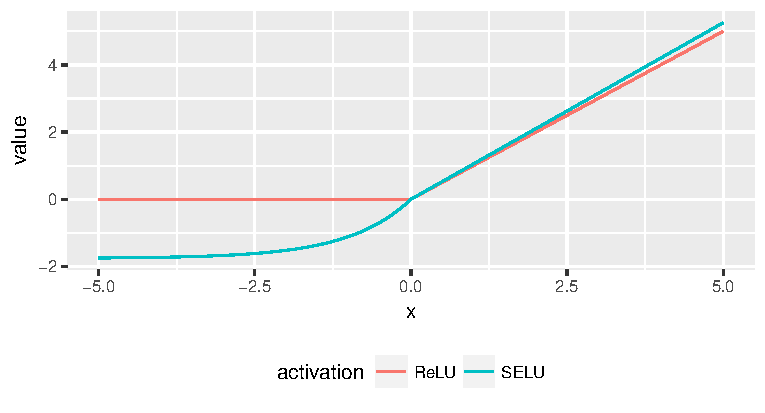
\includegraphics[scale=1]{theory/selu-activation-function.pdf}
    \caption{Shows $\mathrm{ReLU}(x)$ and $\mathrm{SELU}(x)$ in the range $x \in [-5, 5]$.}
    \label{fig:result:selu-bytenet:bytenet-selu-activation}
\end{figure}

The parameters $\alpha$ and $\beta$, are derived from the assumption that the sum $z_{h_\ell}$ approximates a normal distribution. The SELU paper argues that these assumptions are true because of the Lyapunov central limit theorem (CLT). For the Lyapunov variant of CLT to be true, the stochastic variables $z_{h_\ell}, \forall h_\ell \in [1, H_\ell]$ must be independent and the $z_{h_\ell}$ sum must be over many $z_{h_{\ell-1}}$ stochastic variables. The latter is satisfied because the sum is over $H_{\ell-1} k = 2000$ values. However, the former assumption about independence is obviously not true. The SELU paper argues that this is only a weak assumption, as stochastic variables with weak dependencies will still converge to a normal distribution \cite{selu, weak-clt}. Even so, whether or not the weak dependency assumption is satisfied is of course problem and model dependent. The SELU paper shows a big improvement on the MNIST and CIFAR10 dataset using a CNN classifier, which should be considered to be a dataset and model with reasonably high dependencies \cite{selu}.

The initialization should then be done such that $\mathbb{E}[z_{h_\ell}] = 0$ and $\mathrm{Var}[z_{h_\ell}] = 1$. This is achieved by initializing the weights such that:
\begin{equation}
\mathrm{Var}[w_{h_{\ell-1}, h_{\ell}}] = \frac{1}{\mathrm{fan}_{\ell, in}} \quad \Rightarrow \quad r = \sqrt{\frac{3}{\mathrm{fan}_{\ell, in}}}
\end{equation}
where $r$ is the symmetric uniform distribution parameter, similar to that used in He-Initialization. $\mathrm{fan}_{\ell, in}$ is $H_{\ell-1} k$ because the weights are used in convolutional layers.

Using the SELU activation function, as a replacement for the ReLU and normalization layers, and the derived initializer from the SELU activation function, the SELU ByteNet model is created. The ``Memorizing WMT NewsTest'' experiment is then repeated using the SELU ByteNet model. The experiment ran for 150 epochs.

\begin{figure}[H]
    \centering
    \includegraphics[scale=1]{bytenet-selu/validation-memorize-wmt.pdf}
    \caption{Shows BLEU score and cross entropy loss for the German to English WMT NewsTest dataset using the SELU ByteNet. The exponential moving average used a forget factor of $0.1$.}
    \label{fig:result:selu-bytenet:bytenet-selu-wmt}
\end{figure}

The convergence for the ``Memorizing WMT NewsTest'' experiment using SELU ByteNet is somewhat similar to the normal ByteNet case (figure \ref{fig:result:selu-bytenet:bytenet-selu-wmt}). However, there are some significant differences. The initial cross entropy loss is much higher in the SELU ByteNet case, this indicates that the derived initializer isn't the optimal choice. Secondly, the training BLEU score shows almost no improvement initially, then after 75 epochs it improves very fast. These two observations are likely connected, if the initialization is bad it will take a long time for the network to reach a similar state as the normal ByteNet model does initially. If this is true, and if it's possible to initialize the SELU ByteNet model better, the SELU ByteNet model may converge in much fewer iterations than the normal ByteNet model.

Most importantly, the fact that the SELU ByteNet converges much faster than the non-normalized ByteNet model, indicates that the weak-dependency assumptions are sufficiently satisfied. If this was not the case, convergence similarly to that in the non-normalized ByteNet experiment should be expected.

Finally, the synthetic digits experiment using the SELU ByteNet model, shows similar results as the normal ByteNet model (Appendix \ref{appendix:result:bytenet-selu}).

\clearpage
\subsection{Performance Profiling}

Repeating the performance experiment, from both the normal ByteNet model and the simplified ByteNet model, shows that the SELU ByteNet model is extremely fast in comparison. Comparing the time spent running 300 epochs is actually a problem in this case, as the heating phase that transfers data and optimizes allocation takes up most of the time. However, comparing \textit{obs./sec} shows that the SELU model is at least twice as fast as the normal ByteNet model.

\begin{figure}[h]
    \centering
    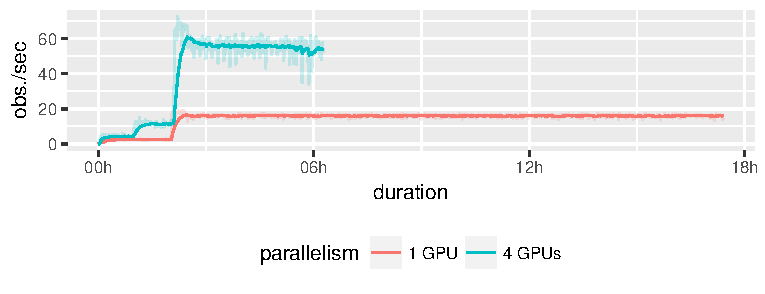
\includegraphics[scale=1]{bytenet-selu/timing-gpus.pdf}
    \caption{Comparing observations per second, depending on the number of GPUs used. The experiment learns the WMT NewsTest dataset over 300 epochs.}
    \label{fig:result:selu-bytenet:timing-gpus}
\end{figure}

The processed profiling in figure \ref{fig:result:selu-bytenet:profile-grouped} (the unprocessed plot is in appendix \ref{appendix:result:bytenet-selu}), shows that the convoluted dilation is the most expensive part. This is completely reasonable, as this is the operation that involves the largest amount of raw computation. However, TensorFlow actually has an inefficient implementation of the dilated convolution, because dilated convolution isn't supported directly by CuDNN v5.1. CuDNN stands for CUDA Deep Neural Network and is a library developed by Nvidia that contains efficient implementations of common operations used in neural networks. The next version of CuDNN supports dilated convolution, but TensorFlow does not yet use this implementation \cite{nvidia-cudnn}.

Another interesting observation when looking at the processed profiling in figure \ref{fig:result:selu-bytenet:profile-grouped}, is the time spent in the ``\textit{pre-normalization}'' layer, which now just contains the SELU activation. Comparing \textit{pre-normalization} to the time spent in \textit{recover-dim}, which just contains a \textit{sequential-dense} layer, shows that the SELU activation uses an unreasonable amount of time. The SELU activation uses less raw computations than the \textit{sequential-dense} layer, and the SELU activation is purely an element-wise operation, thus it should be easy to parallelize. The reason for the poor performance is the before-mentioned naive execution of the computational graph by TensorFlow.

\begin{figure}[h]
    \centering
    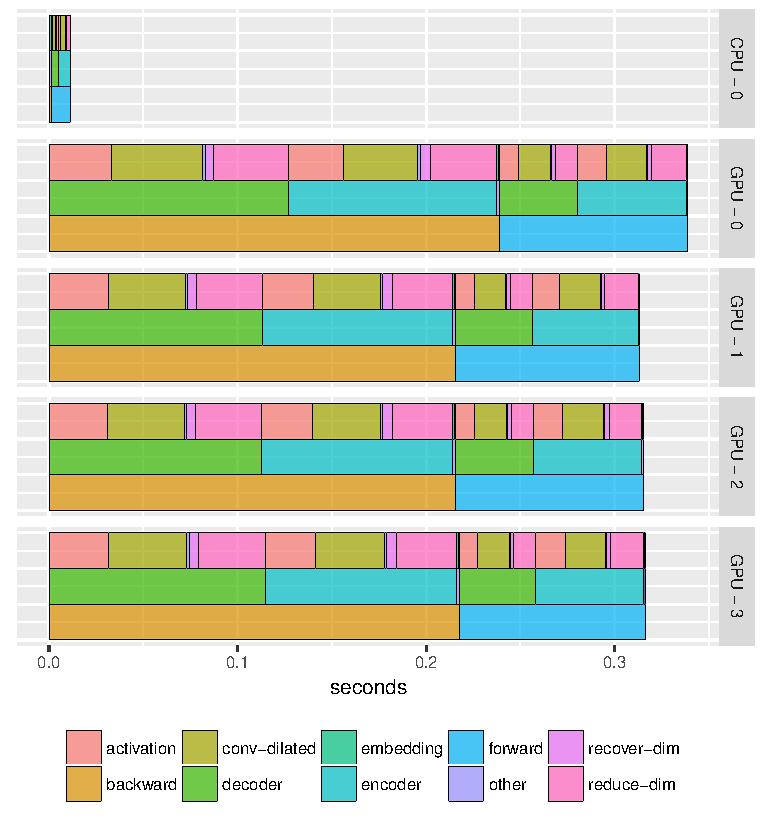
\includegraphics[scale=1]{bytenet-selu/profile-grouped-gpu4.pdf}
    \caption{Shows time spent executing each part of the ByteNet model, this excludes the waiting time. Each part exists in a hierarchy, which is visualized as levels. Bottom level is the backward and forward pass. Second level is the encoder and decoder. Last level primarily splits the SELU ByteNet Residual Blocks.}
    \label{fig:result:selu-bytenet:profile-grouped}
\end{figure}

\clearpage
\subsection{WMT Translation Task}

The Europarl v7 dataset is used to train the SELU ByteNet model. The setup is identical to that previously used to train the normal and simplified ByteNet model.

\begin{figure}[h]
    \centering
    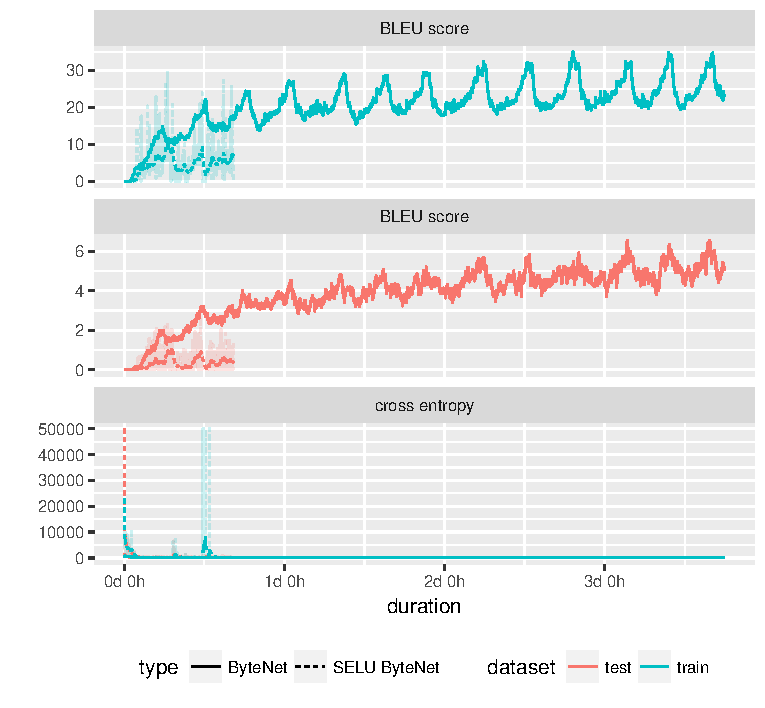
\includegraphics[scale=1]{bytenet-selu/europarl.pdf}
    \caption{Shows BLEU score and cross entropy loss for the SELU ByteNet model, trained on Europarl v7 and tested on WMT NewsTest 2015. Both training and test measures are calculated on a randomly sampled mini-batch from each dataset. The exponential smoothing used a forget factor of $0.05$. The raw data for the non-simplified ByteNet model is not shown.}
    \label{fig:result:bytenet-selu:europarl}
\end{figure}

From figure \ref{fig:result:bytenet-selu:europarl} it is very apparent that the SELU model is extremely fast in comparison to the normal ByteNet model, it completes all 13 epochs in less than a day. However, it also learns extremely poorly.

The cross entropy on the training dataset spikes on occasion, this could explain some of the poor learning behavior. Such an issue is typically solved with gradient clipping, where a hard upper bound is set on the gradient, preventing an exploding gradient. However, the idea behind the SELU activation function is specifically to prevent vanishing and exploding gradients, thus it doesn't seam reasonable to employ additional techniques to prevent exploding gradients.

Another possibility is that the Adam optimization parameters need to be much different when the SELU activation function is used. However, the Adam optimizer acts under most conditions as a trust-region, thus the parameters shouldn't affect the output too much \cite{adam-optimization}.

It is possible that with enough tuning SELU could be made functional, in which case SELU ByteNet would be a very powerful model. However, understanding the behavior of SELU is not easy. The proof for the convergence properties of SELU alone is 90+ pages \cite{selu}. This makes the SELU activation function hard to reason about, thus it is hard to make educated guesses about how to tune the model.

Finally, it is possible that the sparse nature of ReLU is essential for creating a natural language model, where sparse patterns often occur. It is thus possible that the SELU activation function will never work for natural language translation.